%%% Local Variables:
%%% mode: latex
%%% TeX-master: t
%%% End:

\documentclass[bachelor,nofonts]{thuthesis}
%\documentclass[master]{thuthesis}
%\documentclass[doctor]{thuthesis}
% \documentclass[%
%   bachelor|master|doctor|postdoctor, % mandatory option
%   winfonts|nofonts|adobefonts, % mandatory only for bachelor and Linuxer
%   secret,
%   openany|openright,
%   arialtoc,arialtitle]{thuthesis}
% 当使用 XeLaTeX 编译时,本科生、Linux 用户需要加上 nofonts 选项;
% 当使用 PDFLaTeX 编译时,adobefonts 选项等效于 winfonts 选项(缺省选项)。

% 所有其它可能用到的包都统一放到这里了,可以根据自己的实际添加或者删除。
\usepackage{thutils}
\usepackage{tikz}
\usepackage{pgfplots}
\usepackage{algorithm}
\usepackage{algorithmicx}
\usepackage{algpseudocode}
\floatname{algorithm}{算法}
\renewcommand{\algorithmicrequire}{\textbf{输入:}}
\renewcommand{\algorithmicensure}{\textbf{输出:}}

% 你可以在这里修改配置文件中的定义,导言区可以使用中文。
% \def\myname{薛瑞尼}

\begin{document}

% 定义所有的eps文件在 figures 子目录下
\graphicspath{{figures/}}


%%% 封面部分
\frontmatter

%%% Local Variables:
%%% mode: latex
%%% TeX-master: t
%%% End:
\secretlevel{绝密} \secretyear{2015}

\ctitle{基于 Spark 的分布式数据量化与索引系统}
% 根据自己的情况选,不用这样复杂
\makeatletter
\ifthu@bachelor\relax\else
  \ifthu@doctor
    \cdegree{工学博士}
  \else
    \ifthu@master
      \cdegree{工学硕士}
    \fi
  \fi
\fi
\makeatother


\cdepartment[软件]{软件学院}
\cmajor{计算机软件}
\cauthor{文庆福}
\csupervisor{王建民教授}
% 如果没有副指导老师或者联合指导老师,把下面两行相应的删除即可。
%\cassosupervisor{陈文光教授}
%\ccosupervisor{某某某教授}
% 日期自动生成,如果你要自己写就改这个cdate
%\cdate{\CJKdigits{\the\year}年\CJKnumber{\the\month}月}

% 博士后部分
% \cfirstdiscipline{计算机科学与技术}
% \cseconddiscipline{系统结构}
% \postdoctordate{2009年7月——2011年7月}

% 这块比较复杂,需要分情况讨论:
% 1. 学术型硕士
%    \edegree:必须为Master of Arts或Master of Science(注意大小写)
%              “哲学、文学、历史学、法学、教育学、艺术学门类,公共管理学科
%               填写Master of Arts,其它填写Master of Science”
%    \emajor:“获得一级学科授权的学科填写一级学科名称,其它填写二级学科名称”
% 2. 专业型硕士
%    \edegree:“填写专业学位英文名称全称”
%    \emajor:“工程硕士填写工程领域,其它专业学位不填写此项”
% 3. 学术型博士
%    \edegree:Doctor of Philosophy(注意大小写)
%    \emajor:“获得一级学科授权的学科填写一级学科名称,其它填写二级学科名称”
% 4. 专业型博士
%    \edegree:“填写专业学位英文名称全称”
%    \emajor:不填写此项


% 这个日期也会自动生成,你要改么?
% \edate{December, 2005}

% 定义中英文摘要和关键字
\begin{cabstract}
  高维数据的近邻查询是处理多媒体数据的一项重要的技术,在计算机视觉、数据挖掘等
  前沿研究领域有着丰富的应用。随着数据指数式的增长,如何从海量、高维数据中进行尽
  可能快速的近邻查询以及大规模的数据如何存储索引,一直以来都是备受研究者关注的问
  题。
  
  论文的摘要是对论文研究内容和成果的高度概括。摘要应对论文所研究的问题及其研究目
  的进行描述,对研究方法和过程进行简单介绍,对研究成果和所得结论进行概括。摘要应
  具有独立性和自明性,其内容应包含与论文全文同等量的主要信息。使读者即使不阅读全
  文,通过摘要就能了解论文的总体内容和主要成果。
  
\end{cabstract}

\ckeywords{近邻查询, Spark, 向量量化, 倒排索引}

\begin{eabstract}
   An abstract of a dissertation is a summary and extraction of research work
   and contributions. Included in an abstract should be description of research
   topic and research objective, brief introduction to methodology and research
   process, and summarization of conclusion and contributions of the
   research. An abstract should be characterized by independence and clarity and
   carry identical information with the dissertation. It should be such that the
   general idea and major contributions of the dissertation are conveyed without
   reading the dissertation.

   An abstract should be concise and to the point. It is a misunderstanding to
   make an abstract an outline of the dissertation and words ``the first
   chapter'', ``the second chapter'' and the like should be avoided in the
   abstract.

   Key words are terms used in a dissertation for indexing, reflecting core
   information of the dissertation. An abstract may contain a maximum of 5 key
   words, with semi-colons used in between to separate one another.
\end{eabstract}

\ekeywords{\TeX, \LaTeX, CJK, template, thesis}

% 设置 PDF 文档的作者、主题等属性
\makeatletter
\thu@setup@pdfinfo
\makeatother
\makecover

% 目录
\tableofcontents

% 符号对照表
\begin{denotation}

\item[HPC] 高性能计算 (High Performance Computing)
\item[cluster] 集群
\item[Itanium] 安腾
\item[SMP] 对称多处理
\item[API] 应用程序编程接口
\item[PI]	聚酰亚胺
\item[MPI]	聚酰亚胺模型化合物,N-苯基邻苯酰亚胺
\item[PBI]	聚苯并咪唑
\item[MPBI]	聚苯并咪唑模型化合物,N-苯基苯并咪唑
\item[PY]	聚吡咙
\item[PMDA-BDA]	均苯四酸二酐与联苯四胺合成的聚吡咙薄膜
\item[$\Delta G$]  	活化自由能~(Activation Free Energy)
\item [$\chi$] 传输系数~(Transmission Coefficient)
\item[$E$] 能量
\item[$m$] 质量
\item[$c$] 光速
\item[$P$] 概率
\item[$T$] 时间
\item[$v$] 速度
\item[劝  学] 君子曰:学不可以已。青,取之于蓝,而青于蓝;冰,水为之,而寒于水。
  木直中绳。(车柔)以为轮,其曲中规。虽有槁暴,不复挺者,(车柔)使之然也。故木
  受绳则直, 金就砺则利,君子博学而日参省乎己,则知明而行无过矣。吾尝终日而思
  矣,  不如须臾之所学也;吾尝(足齐)而望矣,不如登高之博见也。登高而招,臂非加
  长也,  而见者远;  顺风而呼,  声非加疾也,而闻者彰。假舆马者,非利足也,而致
  千里;假舟楫者,非能水也,而绝江河,  君子生非异也,善假于物也。积土成山,风雨
  兴焉;积水成渊,蛟龙生焉;积善成德,而神明自得,圣心备焉。故不积跬步,无以至千
  里;不积小流,无以成江海。骐骥一跃,不能十步;驽马十驾,功在不舍。锲而舍之,朽
  木不折;  锲而不舍,金石可镂。蚓无爪牙之利,筋骨之强,上食埃土,下饮黄泉,用心
  一也。蟹六跪而二螯,非蛇鳝之穴无可寄托者,用心躁也。\pozhehao{} 荀况
\end{denotation}



%%% 正文部分
\mainmatter

%%% Local Variables:
%%% mode: latex
%%% TeX-master: t
%%% End:

\chapter{引言}
\label{cha:introdction}

\section{研究背景}
在今天这个数据爆炸的时代,文本、图像、视频以及音频等多媒体数据呈现出指数级的增长。如何快速、准确地从这个海量的互联网数据库中获取我们想要的信息,是我们不得不面对的一个问题。Google\footnote{https://www.google.com}、Bing\footnote{http://cn.bing.com}、Baidu\footnote{https://www.baidu.com} 等提供的文本、图像等搜索引擎服务为我们获取信息带来了极大的便利。而在这些搜索引擎背后的都需要用到的一项技术——\textbf{近似近邻查询}(Approximate Nearest Neighbor Search)。在大规模数据的应用场景下,精确的近似查询需要耗费时间太长,不具有实际应用价值。近似近邻查询可以大幅度缩短查询时间,同时保证查询结果与精确查询结果近似,因此更具有实用性。除了信息检索以外,近似近邻查询技术被广泛应用于计算机视觉、机器学习、数据挖掘、模式识别等领域。

在不考虑时间效率的情况下,近似近邻查询问题可以直接通过一种暴力搜索的方式来解决。比如,我们可以直接计算查询数据$q$与数据集合$S$ 中每一条数据的距离,最终根据距离大小,选取出距离最近的前$n$个数据。但在现实中,由于数据集合$S$的规模非常,这种朴素的方法单词查询的计算时间太长而无法采用。但是,如果从规模比较大的数据集合$S$上删选出一个非常小待选集合$S'$,之后再在集合$S'$上进行朴素的暴力搜索选取出前$n$个近邻数据,这时的暴力搜索的时间效率是可以接受的,整个查询过程的时间效率和准确率就取决于删除出待选集合$S'$的过程。待选集合$S'$大小与查询准确率有着密切关系,一般来说,集合$S'$越大,查询准确率越高,但是最终的暴力搜索阶段的时间会变长;集合$S'$越小,则查询效率越低,暴力搜索阶段的时间越短。因此,如何选择一个大小合适、相关性高的待选集合$S'$就成了近似近邻查询问题的关键。

近年来,近似近邻查询问题一直都是研究热点问题之一。目前,这一技术主要面临一下两大挑战:
\begin{enumerate}
\item 海量

随着互联网上的数据越来越多,需要存储的数据量也越来越大。然而,传统的索引结构一般都是基于小规模数据而设计的单机结构。大规模的数据一般无法做到单机存储,更不用说加载到内存当中索引了。这些数据往往存储于分布式系统当中,同时也需要一种分布式的索引结构来支持查询。海量的数据不仅给存储带来了压力,同时也给实时查询带来了巨大挑战。
\item 维度灾难

在多媒体数据处理过程时,往往都会针对多媒体数据提取特征进行处理。为了更好地刻画数据,一般来说,特征数据的维度越高,刻画的准确性也越高。例如,在图像数据处理过程中,我们常常可能用到的 SIFT、SURF 特征都是 128 维的,GIST 特征有 960 维,而 BOVW(Bag of Visual Words)的维度更是高达成千上万维。如此高维度的数据,仅计算两个向量之间距离的时间消耗就比较长,更不必说在大规模数据上进行查询了。
\end{enumerate}

Spark 是一个基于 MapReduce 的通用的大数据并行计算框架,最初由 UC Berkeley AMP Lab 开发。Spark 的架构是在 Hadoop 基础上的改良,继承了 MapReduce 的优点,它与 Hadoop 最大不同之处就是内存计算,Hadoop 将计算过程的中间数据存储在磁盘上,而 Spark 一般是用内存来存储数据,所有数据操作都在内存中完成。

\section{主要研究内容}
本文的主要的关注点是在高维空间中的近似近邻查询问题,通过研究对比现有的几种最新近似近邻查询方法,了解几种不同方法的优缺点。在 Spark 框架下实现了一种基于向量量化(Vector Quantization)的近似近邻查询方法。最终,通过实验来验证算法的准确性以及测试算法时间效率。

\section{论文组织结构}

%%% Local Variables:
%%% mode: latex
%%% TeX-master: t
%%% End:

\chapter{索引结构综述}
\label{cha:related-work}
前文已经提到,近邻查询问题最关键的就是如何选取出一个待选集合$S'$。为了高效地删选出待选集合,我们通常会先把原始的数据索引起来。依据
索引结构的不同,近邻查询的方法可以分为基于树结构的索引和基于哈希的索引。
\section{基于树结构的索引}
\subsection{KD-树}
\subsection{K-Means树}
\section{基于哈希的索引}
基于哈希的索引方法是将高维的数据压缩成二进制编码的形式来进行近似近邻查询,这类方法在图像、文本、视频等多媒体检索上取得不错的效果。
根据哈希函数形式的不同,我们可以简单地将哈希索引分为两类——汉明嵌入和向量量化。
\subsection{汉明嵌入}
汉明嵌入就是要寻找一个映射,对于任意的对象$x \in S$都能映射到二进制串$b(x) \in {0,1}^d$。那么,任意两个对象之间的相似度就可以通过
其对应二进制串之间的汉明距离来近似计算:
\begin{equation}
sim(x, y)\thickapprox 1 - \frac{2\delta_{Ham}(b(x),b(y))}{d}
\end{equation}
\subsection{向量量化}
基于向量量化的哈希索引是对原始向量空间进行量化压缩,原始向量$\mathbf{x} \in \mathbb{R}^D$ 通过量化函数 $q$ 被映射到 $q(\mathbf{x}) \in \mathcal{C} = \{\mathbf{c}_i\}$,其中 $i$ 是下标,$\mathbf{c}_i$ 可以称作为码字,而$\mathcal{C}$则被称为码本。 这种映射可以形式化定义成:$\forall \mathbf{x} \in \mathbb{R}^D$,$\exists \mathbf{c}_i \in \mathcal{C} $,$q(\mathbf{x})=\mathbf{c}_i$。整个量化过程中的量化误差 $E$ 就可以定义为:
\begin{equation}
E = \frac{1}{n}\sum_{\mathbf{x}}\lVert \mathbf{x} - q(\mathbf{x}) \rVert ^2
\end{equation}

其中$\lVert \cdot \rVert$ 表示欧氏距离,而 $n$ 是数据的总量。对于给定的原始数据集合 $S$,我们的目标是找到一个码本 $\mathcal{C}$ 以及对应量化函数 $q(\mathbf{x})$ 使得量化误差 $E$ 最小。在最小化量化误差过程中,不同的限制条件就对应了不同的量化方法。
\subsection{K-Means}
假设有一个包含 $n$ 个 $p$ 维 数据点的集合,$\mathcal{D}\{\mathbf{x}_j\}_{j=1}^n$ , k-means 算法会将这 $n$ 个数据点聚成 $k$ 类,同时用聚类中心来代表每一个聚类的数据。假如矩阵$C \in \mathbb{R}^{p\times k}$的列向量由 $k$ 个聚类构成,每一列都是一个聚类中心,$C=[\mathbf{c}_1,\mathbf{c}_2,\cdots, \mathbf{c}_k]$。k-means 量化的目标函数如下:
\begin{eqnarray}
\mathit{l}_\mathrm{k-means} &=&\sum_{\mathbf{x}\in\mathcal{D}}\min_{i}\lVert \mathbf{x} - \mathbf{c}_i \rVert _2^2 \\
                   &=&\sum_{\mathbf{x}\in\mathcal{D}}\min_{\mathbf{b}\in\mathcal{H}_{1/k}}\lVert \mathbf{x} - C\mathbf{b} \rVert _2^2
\end{eqnarray}

其中$\mathcal{H}_{1/k} = \{\mathbf{b}|\mathbf{b}\in\{0,1\}^k$且$\lVert\mathbf{b}\rVert=1\}$,$\mathbf{b}$ 是一个 1 对 $k$ 编码的二进制向量(包含 1 个 1 ,$k$-1 个 0)。

k-means 量化模型浅显易懂,使用最朴素的近邻查询方法就可以将数据点映射到聚类中心。这种映射过程将每一个原始数据压缩到了 $\log_2k$ 比特的数据,所需要消耗的存储空间随着 $k$ 的线性增长。
\subsection{ITQ}
ITQ(Iterative Quantization)\cite{YunchaoGong:2011:IQP:2191740.2191779}的量化方法是在 2011 年的 CVPR 会议上提出,这一方法较之前的哈希方法在准确率上有了显著提升。

ITQ 方法首先是对原始数据集空间进行 PCA 降维,将原始的 $\mathbb{R}^{n\times d}$ 空间降维成 $\mathbb{R}^{n\times c}$ 空间。此时,再
考虑将降维后的数据集进行二进制编码。从降维后的空间中取出$\mathbf{v}\in \mathbb{R}^{c}$,其对应的编码 sgn($\mathbf{v}$) 可以看做事超立方体$\{-1,1\}^c$
中的顶点。此时,欲使整体的量化误差最小,就是要使原始数据与编码后的数据的欧氏距离最小,$\min{\lVert \mathrm{sgn}(\mathbf{v})-\mathbf{v}\rVert ^2}$。
对于编码前的原始数据集我们用 $X \in \mathbb{R}^{n\times d}$ 来表示,经过 PCA 降维后用 $V \in \mathbb{R}^{n\times c}$ 表示,编码后的数据集用 $B \in \{-1,1\}^{n\times c}$ 来表示。
整体量化误差:
\begin{equation}
Q(B, R) = \lVert B - VR \rVert_F ^2
\end{equation}

其中$\lVert \cdot \rVert_F$ 是 Frobenius 范式,而 $R$ 是正交矩阵,作用是对 $V$ 进行旋转对齐。为何要引入这个旋转矩阵 $R$ 呢?从下图(\ref{fig:itq})可以看出,左侧是 PCA 降维后的数据集 $V$,中间是随机旋转后的数据集,右侧是最优化旋转后的数据集 $VR$。右乘一个旋转矩阵 $R$,让待编码的数据绕数据中心进行旋转到合适状态,每个数据点就可以用距离其最近的数据顶点来表示。下图中可以用 $(-1, -1), (-1, 1), (1, 1), (1, -1) $ 这是四个点来表示。此时,所有的数据点到超立方的顶点的距离和最小,也就是量化误差最小。
\begin{figure}[H]
  \centering
  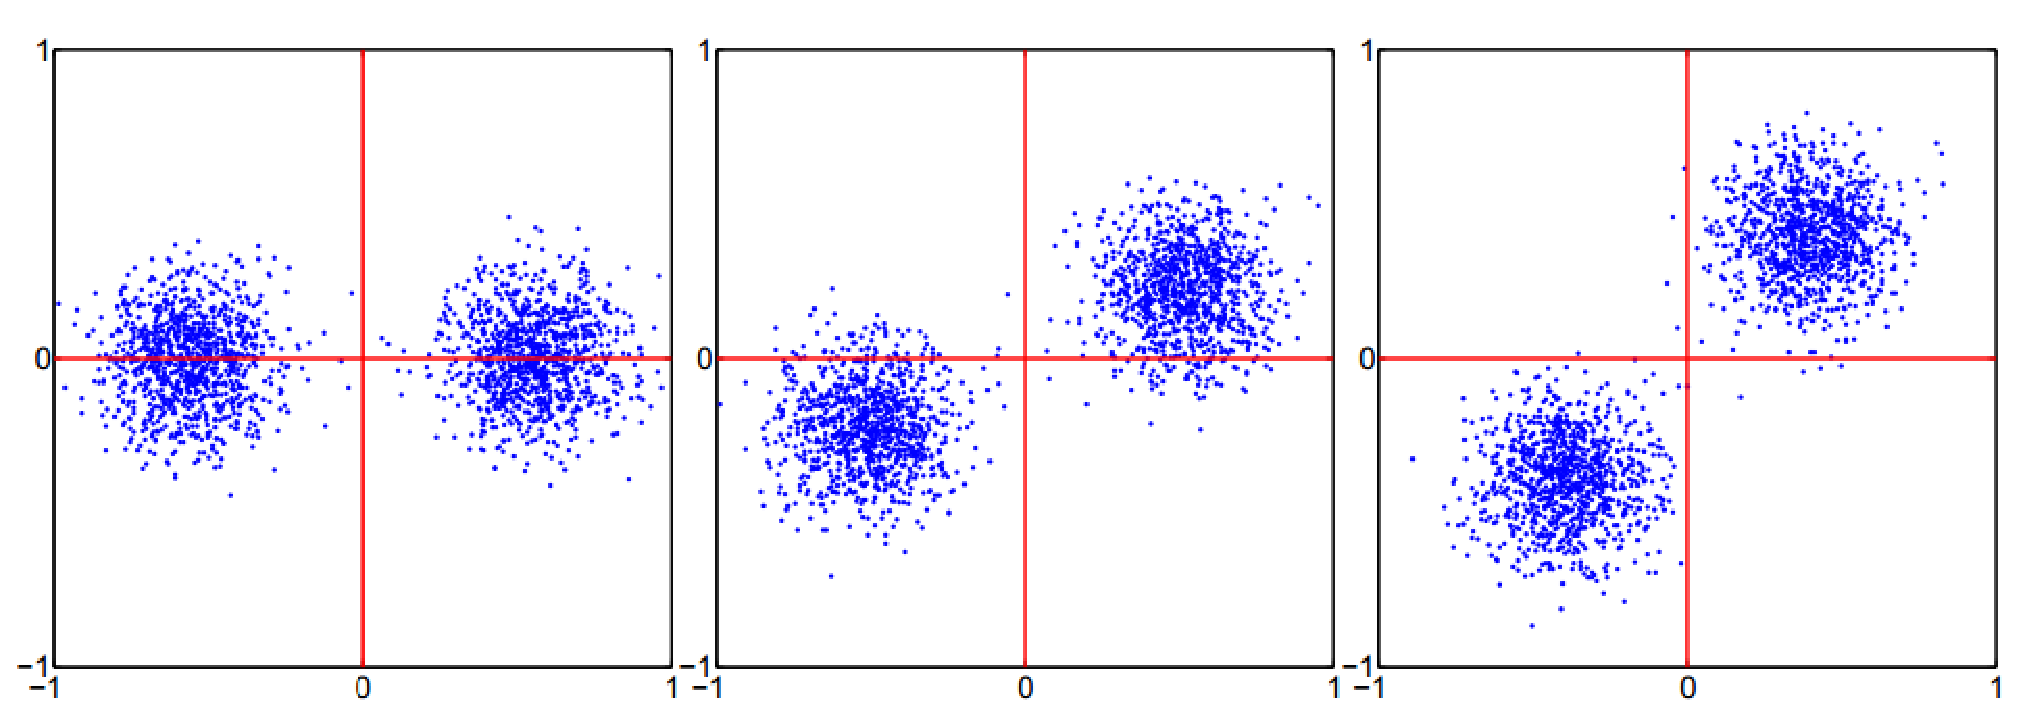
\includegraphics[width=1.0\linewidth]{itq}
  \caption{ITQ 旋转过程}
  \label{fig:itq}
  \footnotesize 注:图像来源\cite{YunchaoGong:2011:IQP:2191740.2191779}
\end{figure}
这样,整个问题的目标函数就变成了$\min \lVert B - VR \rVert_F ^2$。这个公式中有两个未知量,编码后的矩阵 $B$ 和 旋转矩阵 $R$。所以,这个问题的求解要考虑采用交替迭代的方法。先对一个随机生成的矩阵进行 SVD 分解得到一个正交矩阵作为 $R$ 的初始值,此时 $R$ 已知,就可以用$ B= \mathrm{sgn}(VR)$ 来求解 $B$;当 $B$ 已知后,可以对 $B^TV$ 进行 SVD 分解求解 $R$。既然 $R$ 求出,又可以重新一次迭代,固定 $R$ 求 $B$,如此交替迭代就可以求解出该问题。
\subsection{Cartesian K-Means}



%%% Local Variables:
%%% mode: latex
%%% TeX-master: t
%%% End:

\chapter{Spark 弹性分布式数据集与 MLlib 综述}
\label{cha:spark_RDD_mllib}
\section{弹性分布式数据集}
弹性分布式数据集(Resilient Distributed Datasets,下文简称 RDD)\cite{Zaharia2012}是 Spark 中的分布式内存的抽象。相比于 Hadoop 中的计算过程,RDD 可以被缓存在内存当中,每一次的计算产生的结果都可以保留在内存当中。对于迭代计算,这样多次迭代的计算每次可以将结果保存在内存中,下一次迭代又可以直接从内存中读取数据计算,从而避免了大量的磁盘读写操作,大大节省了计算时间。

一般来说,RDD 的创建是通过 SparkContext 来实现,主要包含有两种创建来源:一是从支持的文件系统(或支持的数据库)读取创建;二是从内存数据集合生成。不同于 Hadoop 中仅有 Map 和 Reduce 操作,RDD 还支持其他类型的操作,主要分为转换操作、控制操作和行为操作三类。转换操作顾名思义,就是将一个 RDD 操作之后转换为另一个 RDD,包括 map、flatMap、filter 等操作。控制操作主要用来将 RDD 缓存到内存中或者磁盘上,比如 cache、persist、checkpoint等操作。行为操作主要分为两类:一类是变成集合或标量的操作,另一类是将 RDD 外部文件系统或数据库的操作。Spark 中的所有对 RDD 的操作,只有当执行行为操作时,才会执行之前的转换或控制操作。例如,我们先对 RDD 执行 map 操作, 然后执行 reduce 操作, 在 map 操作时,Spark 并不会真正执行,只是记录,只有执行 reduce 操作时才会真正一起计算。这一特性称为惰性计算(lazy computing)。图(\ref{fig:rdd})展示的 RDD 的一个操作流程。
\begin{figure}[H]
  \centering
  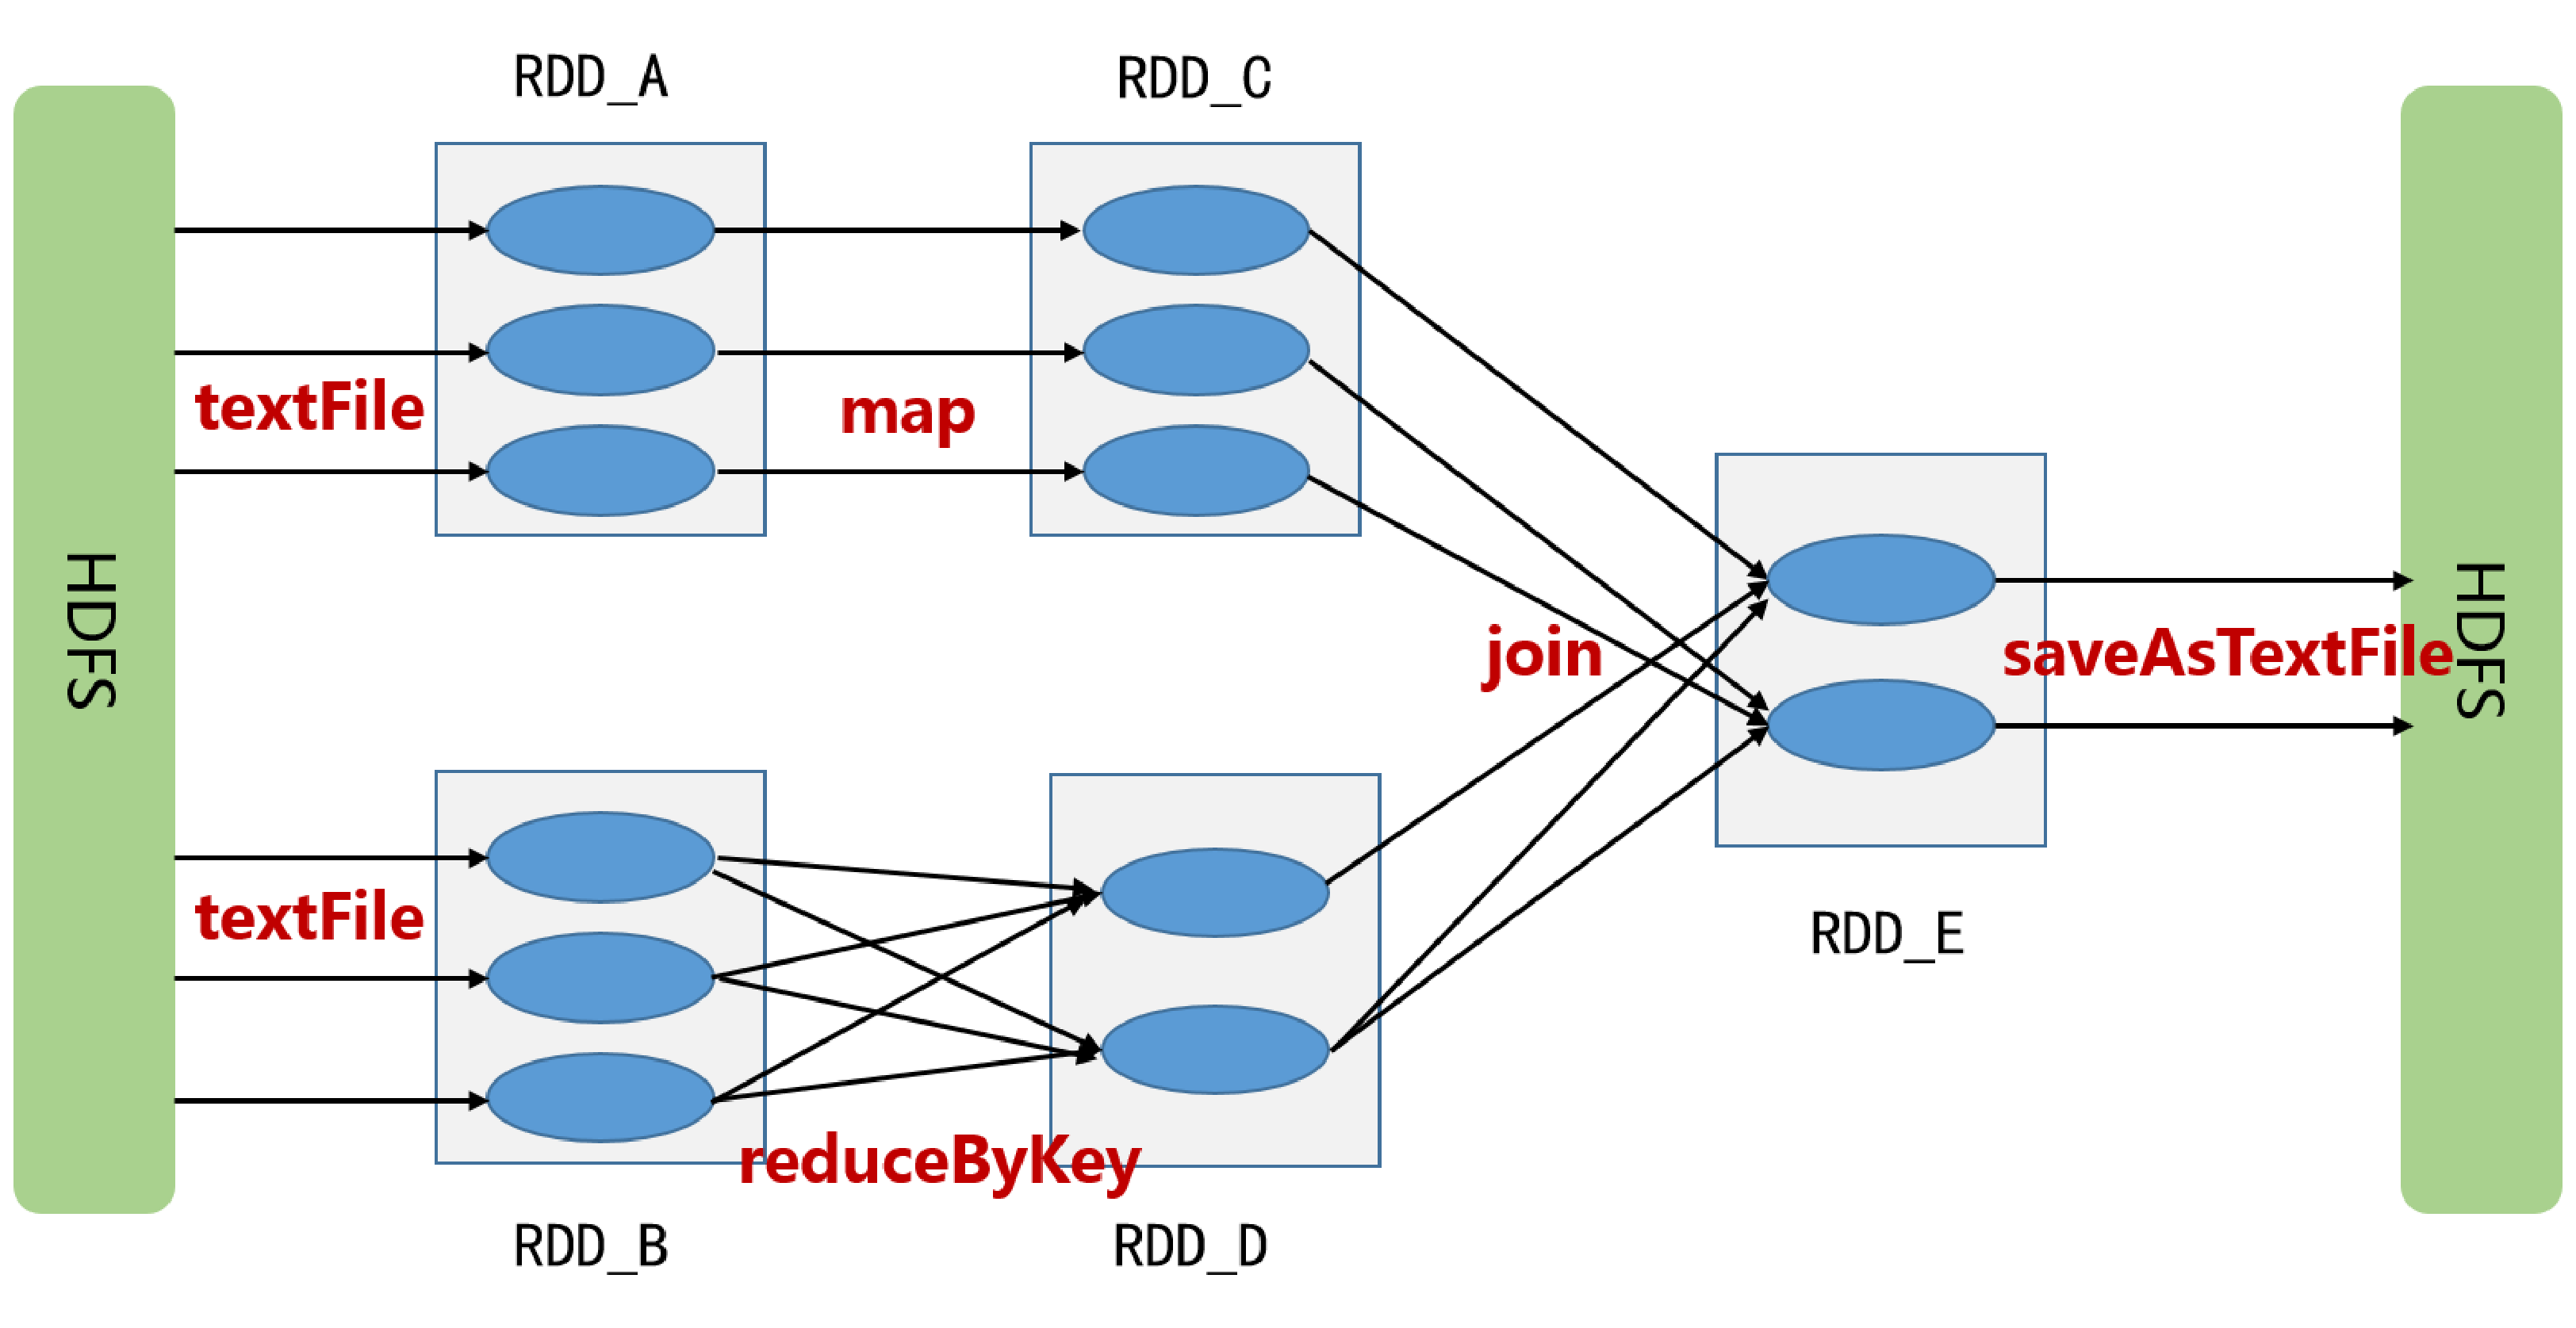
\includegraphics[width=1.0\linewidth]{rdd}
  \caption{RDD 操作流程示例}
  \label{fig:rdd}
\end{figure}
RDD 的持久化是 Spark 中 RDD 的一个重要特性。通过 RDD 的持久化,我们可以将 RDD 缓存到内存或者磁盘上。默认地,RDD 并不会进行缓存,每次计算需要用到 RDD 时,都需要重新计算获取 RDD,这样是非常低效的,特别是对于一些迭代的计算。因此,我们需要考虑在计算过程中,将一些重复用到的 RDD 进行缓存操作,这样我们我们只要第一次计算出 RDD,以后每次用到相同的 RDD 时就不用在重复计算,从缓存中直接读取就可以了。RDD 的 cache() 和 persist() 函数就是用于缓存的,其中 cache() 函数是指将 RDD 缓存在内存当中,而 persist() 根据参数可以将 RDD 进行不同级别的缓存。
RDD 本身自带有容错机制,通过记录 RDD 的演变过程以便在任务执行失败的时候能够恢复出原有的数据,而不需要通过备份的形式实现容错。例如,当前的 RDD 的因任务执行失败而数据丢失,系统则会根据记录的 RDD 演变关系回溯到未丢失的祖先 RDD,重新根据转换操作计算出一个新的 RDD 进行恢复。
\section{MLlib}
随着数据量的不断增大,传统的单机式的机器学习算法实现已经无法满足大数据的要求,分布式机器学习算法是解决大数据机器学习的提供了可能。MLlib 是基于 Spark 构建的一个常用分布式机器学习算法和工具库,目前支持的算法包括分类算法、回归算法、聚类算法、协同过滤算法、降维算法等。MLlib 中的分布式机器学习算法,相比于以往的算法,在时间效率有了明显提升。下图(\ref{fig:logistic-regression})是逻辑回归算法在 Hadoop 和 Spark 上的执行时间对比。
\begin{figure}[H]
  \centering
  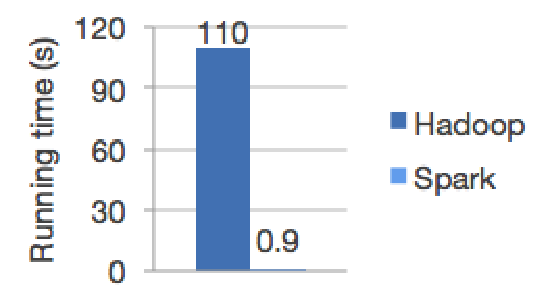
\includegraphics[width=0.3\linewidth]{logistic-regression}
  \caption{Hadoop 和 Spark 上逻辑回归算法效率对比}
  \label{fig:logistic-regression}
  \footnotesize 注:图像来源\protect\footnotemark
\end{figure}
\footnotetext{http://spark.apache.org/}
MLlib 中已经实现的一些常用机器学习算法可以供使用者调用,在 Spark 实现分布式地实现大规模数据的机器学习的任务正是一个不错的选择。



%%% Local Variables:
%%% mode: latex
%%% TeX-master: t
%%% End:

\chapter{基于 Spark 的分布式近似近邻查询系统}
\label{cha:ANNS_based_on_Spark}
\section{乘积量化}
\label{sec:product_quantization}
与之前提到的 K-Means 的量化方法,乘积量化(Product Quantization)\cite{Herve_PQ}也是向量量化的一种。假设我们需要量化压缩 128 维的向量到 64 比特,采用 K-Means 的量化方法的话,需要有 $2^{64}$ 个聚类中心,这样不管是从 K-Means 聚类所需要的时间还是从存储聚类中心所占的空间来看,都是不可行的。

对于上面同样的问题,在乘积量化的算法中,我们首先将原始的数据空间划分为 $m$ 个不相交的子空间,也就是将 128 维的向量切成 $m$ 个长度为 $128/m$ 的子向量。在每个子空间里,分别对子空间中的子向量集合进行 K-Means 聚类,聚类中心数量为 $h$。这样我们就可以用 $1\cdots h$ 这些编号来对子向量进行编码,$m$ 个子向量的编码组合在一起就构成了原始向量的编码。这样,原始空间中一个 128 维的向量就可以压缩到一个 $m\log_2h$ 比特编码表示,从而大大节省了空间。
\begin{figure}[H]
  \centering
  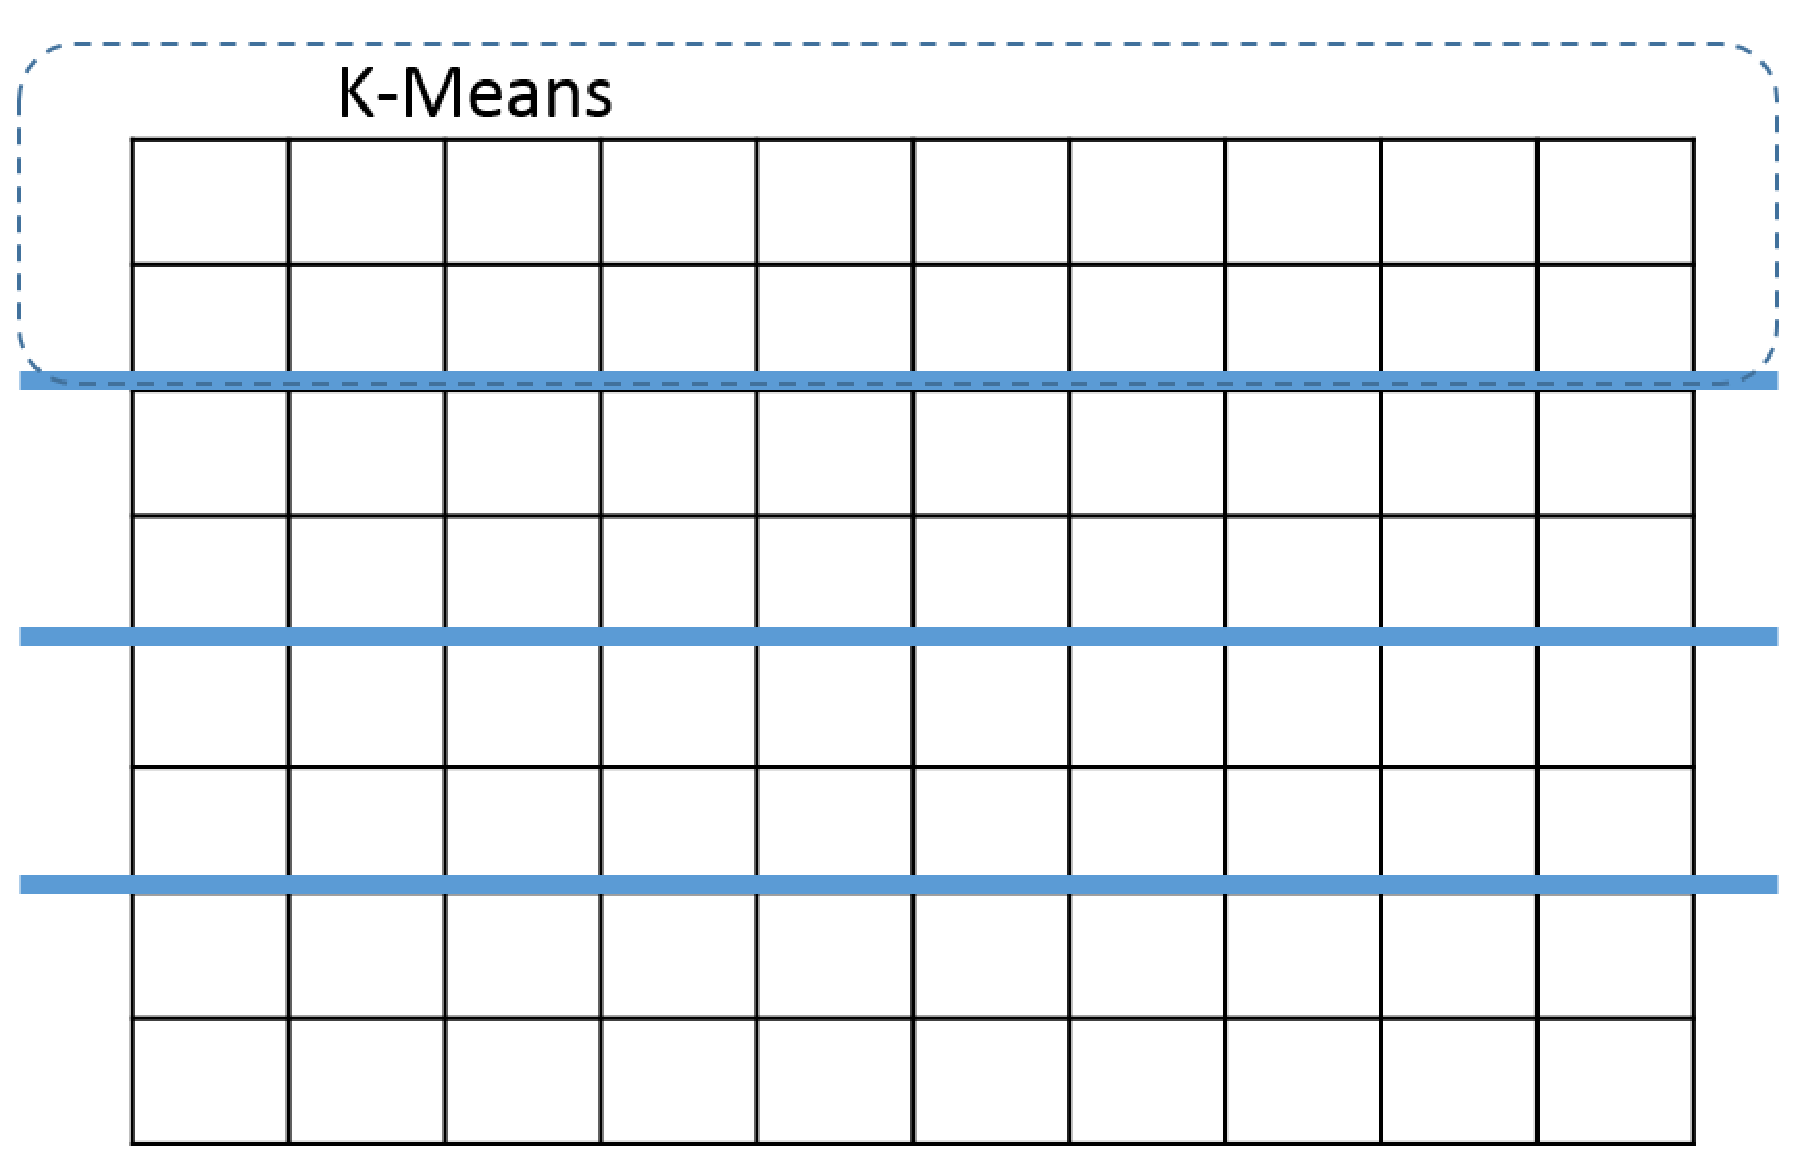
\includegraphics[width=0.5\linewidth]{PQ_subspace}
  \caption{PQ 算法中子空间的划分}
  \label{fig:PQ_subspace}
\end{figure}
更为一般来说,我们可以得到乘积量化方法的目标函数如下:
\begin{equation}
\mathit{l}_\mathrm{PQ} = \sum_{i=1}^n\min\Bigg\lVert \mathbf{x}_i - \begin{bmatrix}C^1\mathbf{b}^1_i\\\vdots\\C^m\mathbf{b}^m_i\end{bmatrix} \Bigg\rVert _2^2
\end{equation}
其中 $\mathbf{x}_i$ 的维度是 $p$,$\mathbf{b}^j_i \in \{0,1\}^h$且$\lVert\mathbf{b}^j_i\rVert=1$,$j \in \{1,\cdots,m\}$。在上面式子中,$C^j(j\in \{1,\cdots,m\})$ 就是我们需要求解的矩阵。在编码过程中,整体的码本(codebook)$C$ 就可以用笛卡尔积的形式表示,$C = C^1 \times \ldots \times C^m$。码本的大小就是所有子空间中聚类中心数量的乘积,根据前面的假设,共有 $m$ 个子空间,每个子空间聚类个数为 $h$,所以码本数量就是 $k = h^m$。求解过程其实并不复杂,正如前文提到,在每个子空间中做 K-Means 聚类就可以求解出码本,这样我们就可以利用码本对每个子空间中的子向量进行编码,从而对原始向量进行编码表示。整个算法的复杂度就和向量维度 $p$、子空间数量 $m$、子空间聚类中心数量 $h$ 有关,存储码本所需要的空间复杂度为 $O(mhp)$。
\begin{table}[htbp]
  \centering
  \caption{乘积量化与 K-Means 量化的空间占用对比}
  \label{tab:kmean_pq}
  \begin{minipage}[t]{0.61\textwidth}
    \begin{tabular}{|c|c|c|c|}
      \hline
                    & 聚类中心 & 编码长度& 空间占用\\
      \hline
      K-Means 量化  &  $k$ &   $\log k$&   $O(kp)$\\
      乘积量化      &   $h^m$ &   $m\log h$ &  $O(mhp)$\\
      \hline
    \end{tabular}\\[2pt]
    \footnotesize 注:$h^m = k$
  \end{minipage}
\end{table}

从表 \ref{tab:kmean_pq} 是乘积量化算法和 K-Means 量化算法的空间占用对可知,当 $m = 1$ 时,乘积量化就退化成普通的 K-Means 聚类量化了。此外, $h$ 取值越大,不仅计算时间复杂度越大,而且空间复杂度也越大,进而也会使得在查询时的时间复杂度变大。因此,选择一个合适的 $m$ 和 $h$ 是非常重要的。论文\cite{Herve_PQ}中指出,$ m = 8 $ 和 $h = 256$ 是比较合适的选择。
\section{利用乘积量化的近似近邻查询}
刚刚我们已经介绍了乘积量化的编码压缩方法,那么如何将这一方法运用在近似近邻查询当中呢?采用乘积量化的方法进行近似近邻查询遵循机器学习类问题的一般流程。整个近似近邻查询算法的主要流程如下:
\begin{itemize}
\item 利用部分数据集,依照乘积量化的方法训练出码本。
\item 在原始的数据集上,采用训练出的码本对其进行编码压缩。
\item 对于任意的查询向量,度量它与编码压缩后的码字之间的距离,从而得到近邻集合。
\end{itemize}
\subsection{训练码本}
首先是训练集的选择,训练集的选取对整个算法是非常关键的,最终近邻查询的准确率一定程度上取决于训练集的好坏。在选择训练集上有两点需要注意,一是训练集的规模大小,二是训练集的代表性。训练集的规模既不宜过大也不能太小,过大会带来过拟合问题,过小则会欠拟合。通常,训练集的规模大小约为原始数据集的 $1/10$ 比较合适。此外,训练集还应该尽可能得有代表性,尽可能广泛地分布于整个数据空间,这样才能使得训练出来的码本能够准确地编码。

在具体训练码本的过程中,如章节 \ref{sec:product_quantization} 中所介绍的一样,首先将训练集中的数据划分到 $m$ 个子空间,在每个子空间中在进行 K-Means 聚类,可以得到聚类中心,也就得到每个子空间的码本。
\subsection{编码压缩}
训练得出每个子空间中的码本之后,将其运用到原始数据集上进行编码压缩。首先,同样也是讲原始数据集划分到 $m$ 个子空间。然后,对于每个子空间中的子向量,分别用训练出来的码本进行编码,也就是用训练好的 K-Means 模型进行预测,可以知道每个子向量隶属于哪个聚类中心,也就知道子向量应该用哪个码字来编码了。这样,整个数据集中的数据都可以用编码来进行表示,存储在内存当中,从而大大节省了空间。
\subsection{近邻查询}

\section{Spark 上的分布式实现}
\subsection{RDD 的划分}




%%% Local Variables:
%%% mode: latex
%%% TeX-master: t
%%% End:

\chapter{总结}
\label{cha:conclusion}
\section{本文工作总结}
本文针对大规模高维数据的近似近邻查询问题,首先对比研究了两大类索引结构——基于树结构的索引和基于哈希的索引。在树结构的索引中,本文介绍了两种用于近似近邻查询的索引树,分别是随机化 KD-树和分层 K-Means 树。在哈希的索引方法中,本文着重介绍谱哈希、K-Means 量化和 ITQ 量化三种哈希方法。在高维空间中,传统的基于树结构的索引方法会使得树的层数随着维度增加而不断增加,空间占用较大。从查询时间上来看,单次查询时间不仅受索引树深度的影响,同时也和查询数据的维度有关。基于哈希的方法对原始空间的数据集进行编码压缩,这类方法不仅减少了数据的占用空间,同时也一定程度上可以提高查询效率。

通过对乘积量化的哈希方法的深入研究,我们在 Spark 平台上实现了一套基于乘积量化哈希方法的近似近邻查询系统。系统中采用基于 RDD 构建的分布式矩阵 BlockMatrix 来存储数据,使用 RDD 的持久化和减少通信数据量来不断优化。最终,通过在 SIFT1M、GIST1M 两个数据集上的实验证明,该系统一方面对数据进行了编码压缩,从而可以大幅度降低空间占用;另一方面在保证查询准确率的同时,通过并行计算的方式可以大大提高查询的时间效率。同时,我们也在 CIFAR-10 数据集上进行图像检索的任务,从而可以看出本系统的实用性。
\section{未来工作展望}
本文已经实现了一套基于 Spark 的近似近邻查询系统,采用乘积量化的方式进行哈希编码,但并没有在 Spark 上实现一套高效的索引方法。目前已被广泛应用的倒排索引方法或是新提出的多重倒排索引方法\cite{BabenkoL12}都是可用于近似近邻查询的索引方法。此外,编码方法也还存在改进的空间,近年来提出的 Cartesian K-Means\cite{Norouzi13} 在乘积量化的基础上,引入了旋转矩阵,在切分的子空间中将数据旋转矫正来减小数据和聚类中心的距离使得编码更加准确,这种方法在检索准确率上比乘积量化更高。

本文的实验是在 SIFT1M、GIST1M、CIFAR-10 三个数据集上进行,未来的工作中可以考虑在 SIFT1B\footnote{http://corpus-texmex.irisa.fr/} 数据集和更大规模的图像或文本数据集上进行实验。最终,可以考虑基于近似近邻查询系统,在一个大规模的真实数据集上构建一个以图搜图的搜索引擎。




%%% Local Variables:
%%% mode: latex
%%% TeX-master: t
%%% End:

\chapter{总结}
\label{cha:conclusion}
\section{本文工作总结}
本文针对大规模高维数据的近似近邻查询问题,首先对比研究了两大类索引结构——基于树结构的索引和基于哈希的索引。在树结构的索引中,本文介绍了两种用于近似近邻查询的索引树,分别是随机化 KD-树和分层 K-Means 树。在哈希的索引方法中,本文着重介绍谱哈希、K-Means 量化和 ITQ 量化三种哈希方法。在高维空间中,传统的基于树结构的索引方法会使得树的层数随着维度增加而不断增加,空间占用较大。从查询时间上来看,单次查询时间不仅受索引树深度的影响,同时也和查询数据的维度有关。基于哈希的方法对原始空间的数据集进行编码压缩,这类方法不仅减少了索引结构的占用空间,同时也一定程度上可以加快了查询效率。

通过对乘积量化的哈希方法的深入研究,我们在 Spark 平台上实现了一套基于乘积量化哈希方法的近似近邻查询系统。系统中采用基于 RDD 构建的分布式矩阵 BlockMatrix 来存储数据,使用 RDD 的持久化和减少通信数据量来不断优化。最终,通过在 SIFT1M、GIST1M 两个数据集上的实验证明,该系统在保证查询准确率的同时,通过并行计算的方式可以大大提高查询的时间效率。同时,我们也在 CIFAR-10 数据集上进行图像检索的任务,从而可以看出本系统的实用性。
\section{未来工作展望}
本文已经实现了一套基于 Spark 的近似近邻查询系统,采用乘积量化的方式进行哈希编码,但并没有在 Spark 上实现一套高效的索引方法。目前已被广泛应用的倒排索引方法或是新提出的多重倒排索引方法\cite{BabenkoL12}都是可用的索引方法。此外,编码方法也还存在改进的空间,近年来提出的 Cartesian K-Means\cite{Norouzi13} 在乘积量化量化的基础上,引入了旋转矩阵,在切分子空间将数据旋转矫正来减小数据和聚类中心的距离使得编码更加准确,这种方法在检索准确率上比乘积量化更高。

本文所进行实验在 SIFT1M、GIST1M、CIFAR-10 三个数据集上进行,未来的工作中可以考虑在 SIFT1B\footnote{http://corpus-texmex.irisa.fr/} 数据集和更大规模的图像或文本数据集上进行实验。最终,可以考虑在一个大规模的真实数据集上构建一个以图搜图的搜索引擎。




%%% 其它部分
\backmatter

\makeatletter
  \listoffigures
  \listoftables
  \listofequations
\makeatother


% 参考文献
\bibliographystyle{thubib}
\bibliography{ref/refs}


% 致谢
%%% Local Variables:
%%% mode: latex
%%% TeX-master: "../main"
%%% End:

\begin{ack}
  衷心感谢导师 xxx 教授和物理系 xxx 副教授对本人的精心指导。他们的言传身教将使
  我终生受益。

  在美国麻省理工学院化学系进行九个月的合作研究期间,承蒙 xxx 教授热心指导与帮助,不
  胜感激。感谢 xx 实验室主任 xx 教授,以及实验室全体老师和同学们的热情帮助和支
  持!本课题承蒙国家自然科学基金资助,特此致谢。

  感谢 \thuthesis,它的存在让我的论文写作轻松自在了许多,让我的论文格式规整漂亮了
  许多。
\end{ack}


% 附录
\begin{appendix}
%%% Local Variables:
%%% mode: latex
%%% TeX-master: "../main"
%%% End:

\chapter{外文资料的书面翻译}
\label{cha:engorg}
\begin{center}
在快速近似近邻查询中选取近邻候选集最高效的方法是什么?
\end{center}
\section{摘要}
近似近邻查询是一项被广泛运用于许多应用场景中的基础而重要的技术。它主要包括两个阶段:选择近邻候选集合和在候选集合进行最朴素的暴力搜索。只有第一个阶段有提升的空间。在现有的大部分方法中,大多是通过将空间近似量化。计算查询数据与被量化的数据(如聚类中心或者比特序列)之前的距离,然后选择适当大小的候选集。这类方法准确性的衡量就是通过在候选集合度量计算来实现。这看似合理但却忽略了一个重要的问题:没有考虑到选取过程的计算时间代价。在本文中,我们提出一种新的近似近邻查询方法,同时关注选取候选集过程的代价。现有的一些方法都用到一些代价比较大的技术,比如说排序或者堆,但我们提出的方法并非如此,是一种非常高效的检索方法。在 $ 10^8$ 的 SIFT 特征数据检索上,相比于现有最好的方法,我们成功减少了 $1/3$ 左右的计算时间。
\section{简介}
给定一个查询数据,查找出与之相近的数据,这就叫做近邻查询。近似近邻查询是在近邻查询基础上的近似。近似近邻查询问题被主动地研究和广泛地应用于许多场景,如近似重复检测、大规模物体识别、文档检索、光学字符识别。近似近邻查询的特点就是在节省时间和空间地情况下准确地找出真正的近邻候选集。在本文中,我们关注于计算效率与准确率之前的关系。

下面我们来讨论一下近邻查询问题中查询准确率与计算时间之前固有关系。如果不考虑计算时间,那么近邻查询问题可以用暴力枚举的方法解决,直接计算查询数据与原有数据之间的距离。因此耗时太长,这种朴素的解决方法并不实用,特别是在处理大数据集时。减少计算时间其实就是要减少最终暴力枚举的数据量。我们先选出一个小的近邻候集合,在这个数据集上进行暴力枚举。只有在选取候选集合的过程需要我们去优化时间效率和准确率。在选取候近邻选集合时,近邻候选集越大,最终查询的准确率就越高,但是这样就会使得最终暴力枚举的时间变长。

目前已有的大多数方法都是通过衡量候选集合的准确性来衡量算法的性能。候选集合的大小决定了暴力枚举的计算时间。然而,选取近邻候选集的过程的计算时间是独立的。因此,忽略掉选取候选集合时间的做法只是觉得了近似近邻查询问题的一部分。

有些文章也适当地考虑了计算时间代价问题。在他们当中,最有效的方法就是多重倒排索引(inverted multi-index,IMI)。然而,在”选取近邻候选集最高效的方法是什么?“这一问题上,我们发现这个问题没有抓住选择近邻候选集过程的本质。下面我们直观上来解释下,假设有 $n$ 个数据,任务是选取近邻候选集,集合大小为 $k$($k<n$)。最差的方法就是将他们全部排序,这需要耗时是$O(n\log n)$。一种更好的方法就是采用有限队列对他们部分排序。这样,每一条数据都被加入到优先队列当中,最终 $k$ 个最近邻的数据留下了。这需要的时间就是 $O(n\log k)$。多重倒排索引用的就是这种方法。然而,还有一种更快的排序方法——桶排序。因为不需要比较序数,它可以在 $O(n)$ 时间复杂度内完成。因此,如果我们能够选择合适的桶,那么选取近邻候选集的过程就可以加快。我们的目标是选取出近邻候选集,所以我们没有必要对桶内的元素按照距离去排序。

对于大规模数据的近似近邻查询问题,我们提出了一种比以往更加高效的近似近邻查询方法。提出的这种方法称为桶距离哈希(bucket distance hashing, BDH)。在实验中,我们在相同平台上比较了这种方法与几种代表性的近似近邻查询方法,分别比较了召回率与计算时间的关系以及召回率与候选集合大小的关系。虽然我们的目标的解决近邻查询问题,但是同样的方法也可以运用到 k 近邻搜索问题当中。
\section{相关工作}
要想高效地选取近邻候选集,通常需要先将数据进行索引。按照索引结构的不同,近似近邻查询方法可以被分为基于树的方法和基于哈希的方法。基于哈希的方法同时也分为数据无关和数据相关两类。前者在索引的过程中不会使用原始数据而后者需要使用。
\subsection{基于树的方法}
FLANN 是一种基于树索引的代表方法。它可以自动选择随机 kd-树,层次 k-means 和暴力枚举中一种最优的方法以及在给定数据集上调参。在实验过程中,我们会将随机 kd-树和层次 k-means 与我们的方法进行比较。
\subsection{基于哈希的数据无关方法}
局部敏感哈希(locality sensitive hashing,LSH)是一种代表性的基于哈希的数据无关的方法。近年来也有很多人对其进行改善。然而众所周知它的性能比数据相关的索引方法要差。此外,拒局部敏感哈希比数据相关的方法也要执行速度上也要慢很多。
\subsection{基于哈希的数据相关方法}
数据相关的方法可以分为在欧氏空间和汉明空间进行选取近邻集合两种。
\textbf{在欧氏空间中选取} \\

这种方法通常使用量化和数据压缩的技术。向量量化(vector quantization,VQ)应用到近似近邻查询中,例如 VQ-index 和 IVFADC。乘积量化(product quantization)被运用在 IMI 当中。正如前面所提到的,IMI 方法要比 IVFADC 方法的效果更好。转换编码被应用在 [3] 中。这一过程可以看做是标量量化(scalar quantization,SQ)。在这个类别中,我们选取 IVFADC 和 IMI 进行比较评价,二者会在下一章节中再介绍。虽然我们实现转换编码,但是它无法和二者比较。
\textbf{在汉明空间中选取}\\

这种方法中,数据通常用二进制编码表示。由于位运算 XOR 操作,这样可以减少内存占用和在汉明空间中的距离计算时间。由于这些好的特性,许多近似近邻查询方法都是基于二进制编码的。在他们当中,谱哈希(spectral hashing,SH)就是一种代表性的方法。

为了实现高召回率的长编码,编码长度为 128 比特或者 256 比特是比较常见的。其实处理这么长的编码是不简单的。在汉明空间中选取近邻候选集合的基准方法是顺序查找。这种方法虽然很快,但却无法再大数据集上应用。有人也许认为树结构或哈希结构能够实现子顺序查找。然而,在汉明空间进行等距离数据的查找,随着距离增大,查找的数据量会呈现出爆炸增长。这使得选取近邻候选集的过程变得不太高效。正如 [16] 中之处一样,使用原始的 LSH 来哈希。然而前面提过,数据无关的方法并不高效。另一个也许稍微复杂一点的方法就是现有的在欧氏空间的近似近邻查询方法。我们将自己提出的方法运用在谱哈希上。但是,并没有将其与现有的代表性方法进行比较。
\section{现有基于向量和乘积量化的哈希方法}
回顾一下 IVFADC 和 IMI 方法可以帮助更好地理解我们提出的方法 BDH。因此在这一章节,我们会比第二章中更加详细介绍他们。
\subsection{IVFADC}
IVFADC 使用 VQ 索引数据可以高效地选取近邻候选集,使用 k-means 聚类算法将数据分成许多个聚类。给定一个查询数据,与之相近的聚类会被检索到,隶属于该聚类的所有数据会被选为近邻候选集。这有可能使得有些数据与查询数据近邻却没有被选取到近邻集合中。然而在相同聚类中心数量下的量化误差最小,VQ 被认为是最好的量化方法。
\subsection{多重倒排索引}
作为比 IVFADC 更好的解决方法,Babenko 和 Lempitsky 提出的 IMI 使用乘积量化代替向量量化。PQ 是一种介于 SQ 和 VQ 之间的量化方法。向量空间被划分成很多个子空间,之后再每个子空间上运用 VQ 编码。在相同数量的聚类中心下,PQ 一般会产生比 VQ 更大的量化误差。然而为了达到相同召回率,计算时间可以通过多序列算法(MSA)来减少。
\begin{figure}[H]
  \centering
  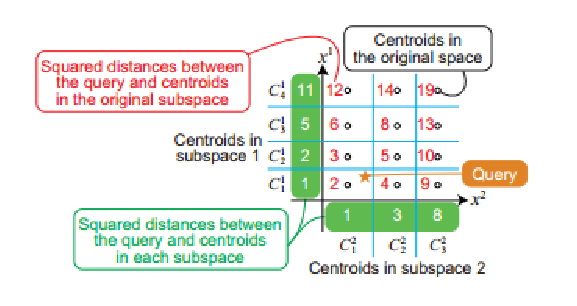
\includegraphics[width=0.5\linewidth]{f_imi}
  \caption*{IMI 算法的介绍}
  \label{fig:f_imi}
\end{figure}
上图中回顾介绍了 IMI 算法。根据图片所示,在子空间 1 中有 4 个聚类中心,在子空间 2 中有 3 个聚类中心。聚类中心的用 $C_j^i$ 表示,其中 $i$ 表示子空间标号,$j$ 表示第 $i$ 个子空间中的聚类标号。首先,计算用星号表示的查询数据与子空间聚类中心之间的平方距离。原始的平方距离是每个子空间中的平方距离之和。然后,如果在原始空间中的所有距离都计算完了,中心离查询数据近的就会被查找出。但是,没有必要去计算在原始空间中所有的距离。因为子空间中的中心距离大的中心并不能在过程中发挥作用。因此,他们在 MSA 算法中被忽略不计。
\begin{figure}[H]
  \centering
  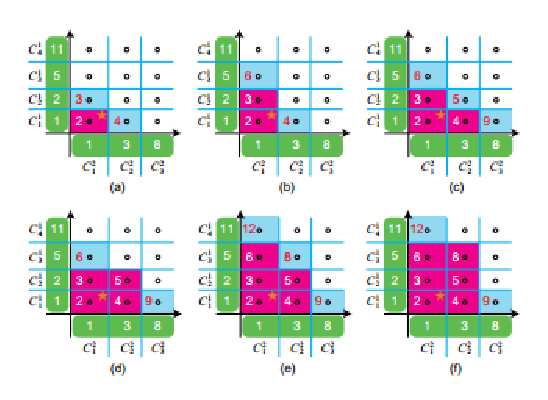
\includegraphics[width=0.5\linewidth]{f_msa}
  \caption*{MSA 算法的介绍}
  \label{fig:f_msa}
\end{figure}
图中是 MSA 算法的概览。在 MSA 算法中,每个子空间中的平方距离事先被排序好了。然后,子空间的中心按距离递增顺序一次排列。正如 图(a)所示,第一个查找的聚类就是 $C_1^1 \times C_1^2$ 的积,与查询数据的距离为 2。相邻的聚类中心 $C_2^1 \times C_1^2$ 和 $C_1^1 \times C_2^2$ 会在下一次中作为候选集被查找出。

如上所示,MSA 算法比较聚类中心之间的距离并将其按照升序排列。这在近邻查询中是不必要的。在这点上,这种方法就没有抓住近邻查询的本质。图中描述了子空间数量为 2 的情况。如果空间划分多于 2 的话,那么整个计算的代价就会变大。因此,IMI 算法最佳情形就是子空间数量为 2。我们将会展示子空间被划分成多余 2 同时获得更好的查询效率的算法。
\section{提出的方法}
\subsection{回顾}
正如第一章节中所提,我们提出的方法最关键的想法就是在选取近邻候选集的时候不做数据的排序。我们采用分支定界法来代替 MSA 算法解决相同问题。
\begin{figure}[H]
  \centering
  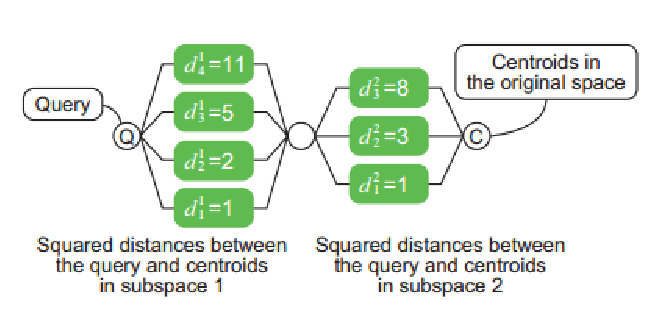
\includegraphics[width=0.5\linewidth]{f_distance}
  \caption*{子空间的距离计算}
  \label{fig:f_distance}
\end{figure}
图中,介绍了我们所提出的算法。图中绘制了查询数据(Q)和聚类中心(C)路径。路径的左右半边分别表示在查询数据和聚类中心之间子空间 1 和子空间 2 中的平方距离 $\{d^i_j\}$。$d^i_j$ 和 $C^i_j$ 的标号示意相同。然后,我们会确定平方距离的上界。整个过程中,上界会不断地增大。在所有路径中,距离小于上界的聚类中心就会被查找出来。
\begin{figure}[H]
  \centering
  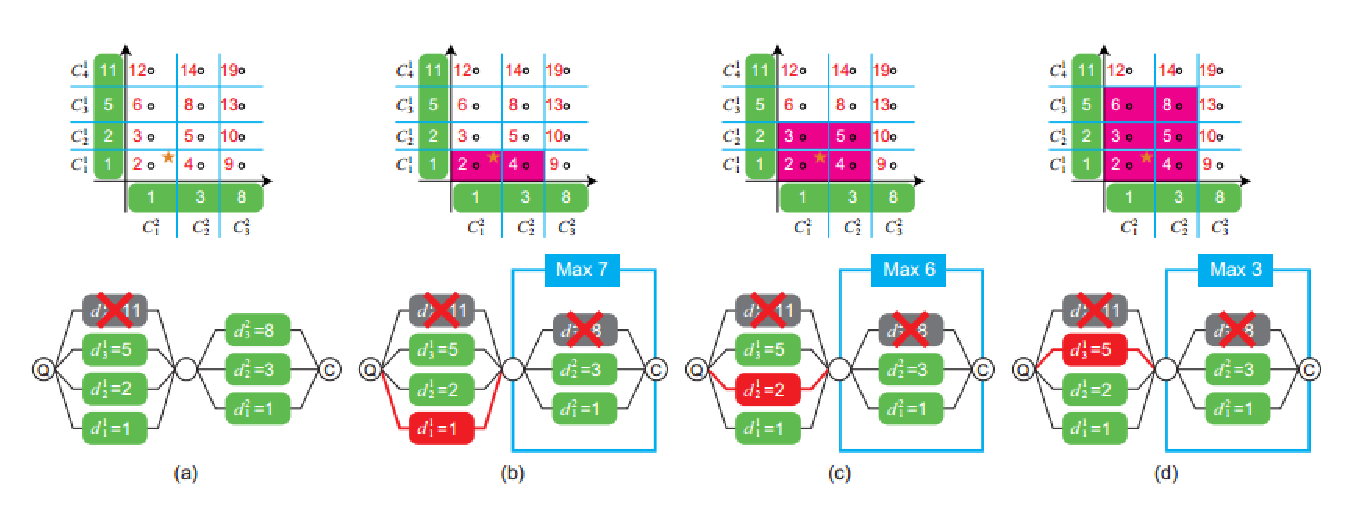
\includegraphics[width=\linewidth]{f_bdh}
  \caption*{BDH 算法示意图}
  \label{fig:f_bdh}
\end{figure}
图中描述了提出的算法流程,平方距离的上界是 8。整个算法流程从(a)到(d)。在(a)中,当上界被设置成 8,路径 $d^1_4 =11$ 就会立即被删除。之后,子空间 1 中的每条路径都会遍历一遍。在(b)中,路径 $d^1_1$ 被遍历。由于上界是 7,路径上子空间 2 中 $d^2_1 =1$ 和 $d_2^2=3$ 会被选出到近邻候选集。在(c)中,$d^1_2$ 被遍历,由于上界是 6,路径上子空间 2 中 $d^2_1 =1$ 和 $d_2^2=3$ 会被选出到近邻候选集中。
\subsection{准备}
为了更详细地解释我们提出的方法,需要提前做一些定义。我们假设,查询数据 $q$ 和待查询数据集都用向量表示。用 $N$ 和 $D$ 分别表示待查询数据的数量和维度。我们会在待查询数据集上进行 PCA 降维以减小距离度量的误差和获取最大的 $u$ 个主成分(特征值)降序的 $l_1,l_2,\ldots,l_u$。用$\mathbf{V}=[v_1 v_2 \cdots v_u]$ 表示与 $u$ 个特征值对应特征向量组成的矩阵。$u$ 对应多维哈希表的维度。我们之后会介绍一种自动确定 $u$ 大小的算法。
\subsection{索引与调参}
PQ 将特征空间划分成 $p$ 维的子空间。例如,一个 $u$ 维的向量 $\mathbf{x}$ 被 $u$ 个特征值表示为 $\mathbf{x} = \{x_1,\ldots,x_m\}$,其中 $m = u/p$。然后,在 $p$ 维的子空间上进行 k-means 聚类。

除去 $p$ 以外,我们提出一套自动调参的算法。首先,我们开始为聚类算法进行自动调参选择。目标是要将待查询数据集在第 $i$ 个子空间聚类成 $k_i$ 个类,得到所有 ${k_i}$ 以及每个子空间中的聚类中心。用$x_{is}$表示第 $s$ 条数据的第 $i$ 个子向量,用 $C_j^i$ 表示第 $i$ 个子空间中的第 $j$ 个聚类中心。然后量化误差第 $i$ 个子空间的$E_i$定义如下:
\begin{equation*}
E_i = \sum_{s=1}^N\left( x_{is} - C^i_{q_i(x_{is})}\right)^2
\end{equation*}
其中 $q_i(x)$ 函数定义如下:
\begin{equation*}
q_i(x) = \arg\min_{j} \left( x - C^i_j\right)^2
\end{equation*}
因为过大的量化误差会导致距离度量时的误差过大,所以我们要采取策略使得子空间中的 $E_{max}$ 最小。算法 1 介绍了我们提出的算法。它会增加具有最大量化误差的子空间中聚类中心的数量,并在当桶的总数量达到待查询数据的数量时结束。这样,特征空间就会被分成 $N_{bkt}$ 个桶,对应到多维哈希表的哈希大小。通过对人造数据和真实数据的实验中,我们可以找到算法的终止条件。

这个算法同时也可以确定多维哈希表的维度 $u$。如果在子空间 1 中有 $k_i$ 个聚类中心,那么子空间中的量化误差就小于 $E_{max}$。假如子空间不需要划分,假设特征值被降序排列,对于 $i=1,\ldots,m'$,现有的 $m'$ 满足 $k_i > 1$ 而且对于 $i=m'+1,\ldots,\lfloor D/p\rfloor$ 有 $k_i=1$。然后可以忽略后半部分($i>m'+1$),$u$ 设置为 $m'p$。
\subsection{高效选取近邻候选集合}
用 $c$ 表示近邻候选集的集合大小。我们提出的算法可以一步一步地选择至少 $c$ 个最近距离的候选数据。算法 2 和算法 3 展示了整个详细过程。其中有一部分在章节 4.1 中已经有所介绍了。算法 2 可以找到距离在下界 $L$ 和上界 $U$ 之间的桶。$L$ 和 $U$ 的初始值分别是 0 和 查询数据与最近桶之间的平方距离。只要当前选取的近邻候选集大小 $n$ 小于 $c$,整个过程会一直循环执行。$\Delta$ 表示 $L$ 和 $U$ 的增量,我们设置 $\Delta$ 的大小为特征值之和的 $1/100$。
\section{实验}
我们通过实验对比提出的方法(BDH)与一些代表性的近似近邻查询算法,包括 IVFADC 和 IMI。所有方法都用 C++ 语言实现。我们依照 MATLAB 版本的 IVFADC 和 C++ 源码 IMI 算法实现基于哈希的方法。 IVFADC、IMI 和 BDH 共用大部分的代码。这样可以避免在实验过程中的差异并且尽可能公平地对比。对于基于树的方法,我们使用 C++ 源码实现的 FLANN。FLANN 自身无法使用于大数据集合。我们通过实验探索每种方法的最佳参数设置。实验中的参数设置见表格。
\begin{table}[htbp]
  \centering
  \caption*{实验中的参数设置}
  \label{tab:f_parameters}
  \begin{minipage}[t]{\linewidth}
    \begin{tabular}{|c|c|c|c|c|c|c|c|}
      \hline
        Methods  & 参数 & SIFT1M& SIFT10M& SIFT100M& GIST1M&GIST10M\\
      \hline
      BDH  &  $\log_2|C|,P$& 20,5 & 26,3 & 28,5 & 22,5 & 24,5\\
      \hline
      IMI  &  $\log_2|C|$  & 14 & 18 & 20 & 18 & 22\\
      \hline
   IVFADC  &  $\log_2|C|$  & 10 & 12 & 14 & 12 & 14\\
    \hline
      RKD  &  $No.of trees$& 8  &  8 &  8 &  8 & 16\\
      \hline
      HKM  &  $k$          & 32 & 64 &  N & 64 & 32\\
      \hline
    \end{tabular}
  \end{minipage}
\end{table}
我们使用包含 10 亿个 128 维 SIFT 特征描述符的 BIGANN 数据集和包含大约 8 亿 384 维 GIST 特征描述符的 80 Million Tiny Images。对于前者,我们使用 1M、10M、100M 大小的数据集,1000 个向量用来做查询。对于后者,我们使用 100K、1M、10M 大小的数据集。对于两类数据,都是用最小的数据集来做训练。

我们使用有 4 CPUs(AMD Opteron 6174,2.2GHz,12 cores)和 256G 内存的服务器来运行实验。所有的数据都存储在内存当中。所有的程序都是单核单线程执行。
\subsection{实验 1:召回率与计算时间}
我们通过召回率与计算时间关系比较了所有的算法。计算时间是平均一次查询所需要的计算时间。由于计算时间限制,计算时间少的准确率相比之下比较低。图中显示了在 SIFT 和 GIST 数据集上的实验结果。从实验结果看出,我们提出的方法比其他方法的效果都要好很多。其中图(c) 中显示在召回率为 90\%时, BDH 算法是 IMI 算法的两倍快,是 IVFDC 的 4.5 快;在召回率为 60\%时,BDH 算法是 IMI 的 2.9 倍快,是 IVFADC 的 9.4 倍快。比较图(a)到图(c),提出的方法的优点随着数据集增大就越明显了。这显示出这个算法的可扩展性好。相反,比较图(d)到图(f),提出的方法的优点并没有变化。

IVFADC 和 IMI 无法扩展是因为相对大规模计算代价。用 $G$ 表示原始空间中的聚类数量, IVFADC 在选择近邻候选集时需要 $O(G)$ 时间来计算距离。IMI 需要 $O(2\sqrt{G})$ 计算距离,需要 $O(\sqrt{G}\log\sqrt{G})$ 在子空间中排序。
\begin{figure}[H]
  \centering
  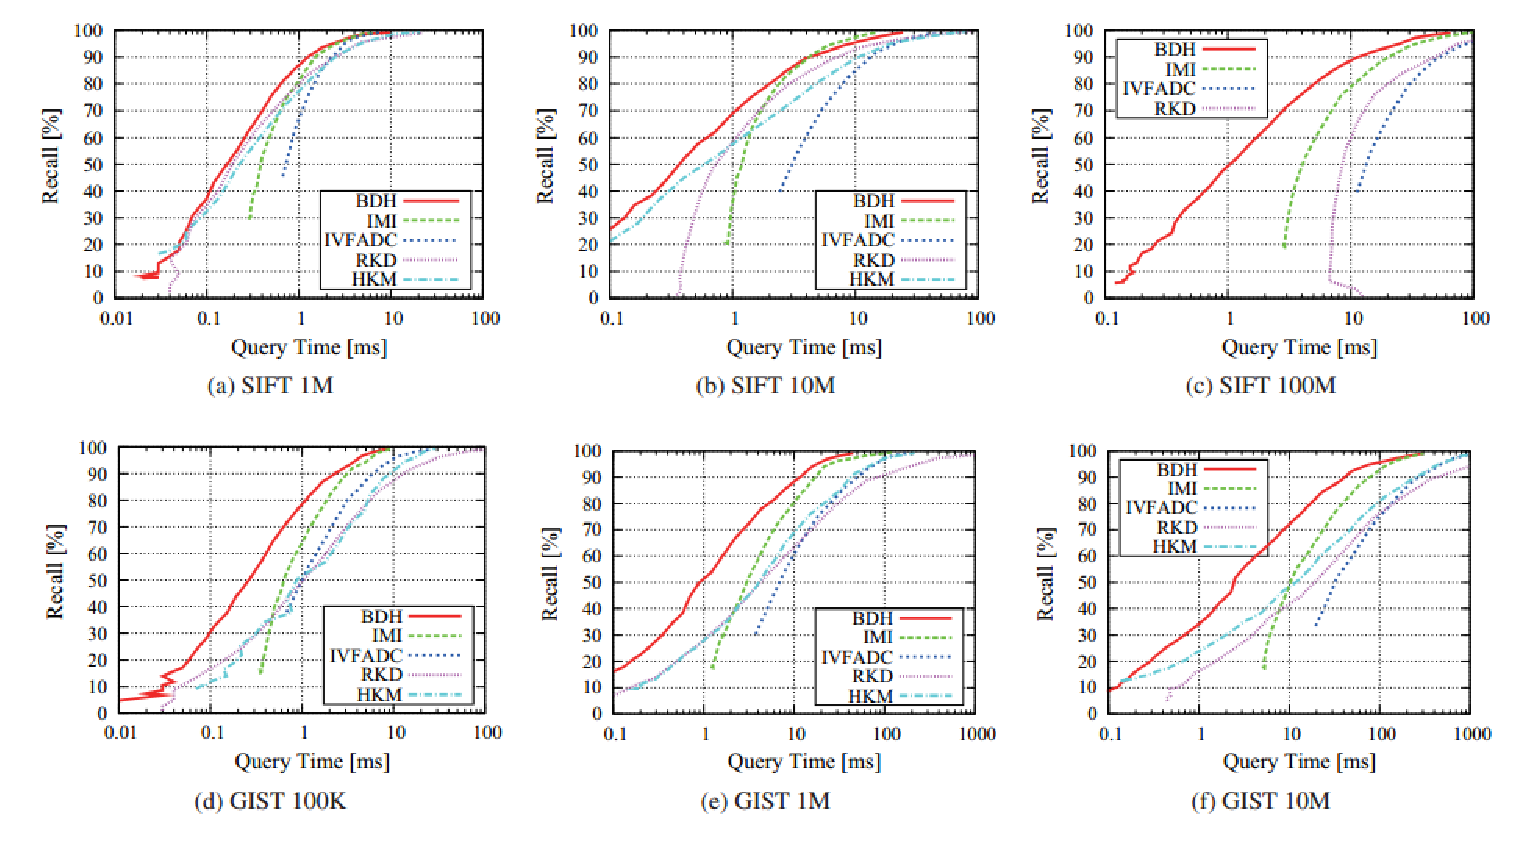
\includegraphics[width=\linewidth]{f_experiments}
  \caption*{实验结果图}
  \label{fig:f_experiments}
\end{figure}
\subsection{实验 2:召回率与候选集大小}
我们同时也通过召回率与候选集大小的关系来比较所有算法。为了适合这个标准,我们选择最佳的参数来进行实验。通过图中可以看到,我们的方法要比 IVFADC 和 IMI 方法好。
\begin{figure}[H]
  \centering
  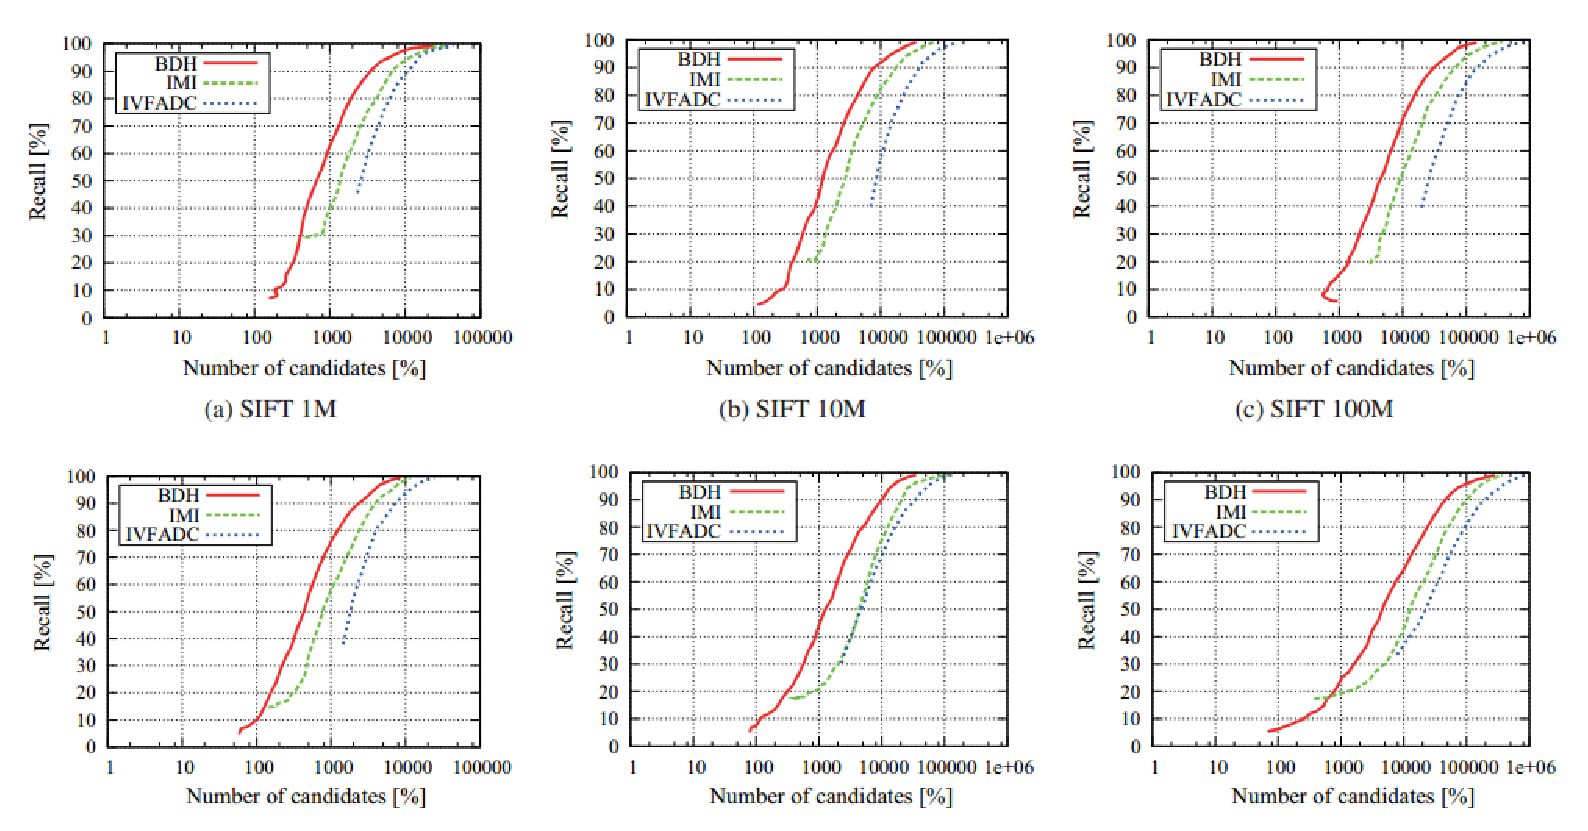
\includegraphics[width=\linewidth]{f_experiments2}
  \caption*{实验结果图 2}
  \label{fig:f_experiments2}
\end{figure}
\section{结论}
在近似近邻查询的过程中,只有选择近邻候选集的过程可以变改善。在本文中,我们指出了衡量近似近邻查询算法的计算代价的重要性。计算代价是近似近邻查询算法的衡量中必不可少,研究者忽略计算时间的方法是有缺陷的。我们发现,目前最好的近似近邻查询算法 IMI 并没有把我到选取近邻候选集合的本质。因为近似近邻查询算法只需要选出最近邻的候选集合,所以没有比较去做排序。

最后,我们提出一种新的将计算代价考虑在内的近似近邻查询算法。这种方法基于分支定界算法,可以进行非常高效地检索。我们也提出一种自动调节参数的算法,除了一个参数以外,其余参数可以自动调节到最好。在 100M SIFT 特征实验中,相比于现有最好的算法,我们提出的算法在减少三分一左右的计算时间。在召回率为 90\% 和 60\% 时,分别是最好算法的 2 倍 和 2.9 倍快。
\begin{center}
\textbf{书面翻译对应的原文索引}
\end{center}

\begin{enumerate}[{$[$}1{$]$}]
\item Iwamura M, Sato T, Kise K. What is the most efficient way to select nearest neighbor candidates for fast approximate nearest neighbor search? The IEEE International Conference on Computer Vision (ICCV), 2013
\end{enumerate}

\end{appendix}

\end{document}
